\documentclass{article}
\usepackage{graphicx} 
\usepackage{amsmath}
\usepackage{amssymb} 

\usepackage{hyperref}
\usepackage{parskip} 

\usepackage{endnotes}

\usepackage[utf8]{inputenc} 
\usepackage[ngerman]{babel} 
\usepackage[T1]{fontenc}   



\title{Abgabe 1 für Computergestützte Methoden}
\author{Gruppe 15: Dania Khudeda (4347860), Arany Mahendran (4335991), \\
Lea Kryzecki (4340237)}


\date{1. Dezember 2024}

\begin{document}
\maketitle 
\tableofcontents
\newpage
\section{Der zentrale Grenzwertsatz}

Der zentrale Grenzwertsatz (ZGS) ist ein fundamentales Resultat der Wahrscheinlichkeitstheorie, das die Verteilung von Summen unabhängiger, identisch verteilter $(i.i.d.)$ Zufallsvariablen (ZV) beschreibt. 
Er besagt, dass unter bestimmten Voraussetzungen die Summe einer großen Anzahl solcher ZV annährend normalverteilt ist, unabhängig von der Verteilung der einzelnen ZV. Dies ist besonders nützlich, da die Normalverteilung gut untersucht und mathematisch handhabbar ist.

\subsection{Aussage}

Sei $X_1$, $X_2$,..., $X_n$ eine Folge von $i.i.d.$ ZV mit dem Erwartungswert $\mu = \mathbb{E}(X_i)$ und der Varianz $\sigma^2$ = Var$(X_i)$ , wobei 0 < $\sigma^2$ < $\infty$ gelte. Dann konvergiert die standardisierte Summe $Z_n$ dieser ZV für ${n \to \infty}$ in Verteilung gegen eine Standardnormalverteilung:\footnote[1]{Der zentrale Grenwertsatz hat verschiedene Verallgemeinerungen. Eine davon ist der \textbf{Lindeberg-Feller-Zentrale-Grenzwertsatz} \cite{buch}, Seite 328], der schwächere Bedingungen an die Unabhängigkeit und die identische Verteilung der der ZV stellt.}

 \begin{equation}
 \label{eq: sum}
     Z_n = \frac{\sum_{i=1}^{n} X_i - n\mu}  {\sigma\sqrt{n}}\overset{d}\to \mathcal{N}(0,1). 
 \end{equation}


Das bedeutet, dass für große $n$ die Summe der ZV näherungsweise normalverteilt ist mit Erwartungswert nµ und Varianz $n\sigma^2$: 

\begin{equation}
    \label{eq: sum1}
 \sum_{i=1}^{n} X_i \sim\mathcal{N}(n\mu, n\sigma^2).
\end{equation}

\subsection{Erklärung der Standardisierung}

Um die Summe der ZV in eine Standardnormalverteilung zu transformieren, subtrahiert man den Erwartungswert $n\mu$ und teilt durch die Standardabweichung $\sigma \sqrt{n}$. Dies führt zu der obigen Formel \eqref{eq: sum}. Die Darstellung \eqref{eq: sum1} ist für ${n \to \infty}$ nicht wohldefiniert.

\subsection{Anwendungen}

Der ZGS wird in vielen Bereichen der Statistik und der Wahrscheinlichkeitstheorie angewendet. Typische Beispiele sind:
\begin{itemize}
    \item  Beim Werfen eines Würfels wird der Drurchschnitt der Augenzahlen bei vielen Würfen näherungsweise normalverteilt, obwohl die Einzelwerte diskret sind.
    \item Die Summe der täglichen Kundenzahlen über viele Tage ist näherungsweise normalverteilt, unabhängig von der Verteilung an einem einzelnen Tag.
    
\end{itemize}

\newpage
\section{Bearbeitung zur Aufgabe 1}
\subsection{Thema Datenverarbeitung}
\begin{enumerate}
\item Untersuchen Sie den für Ihre Gruppe relevanten Teil der Daten, um sich mit seinem Aufbau vertraut zu machen, und beschreiben Sie Ihre Erkenntnisse:

Bei der CSV-Datei (Comma Seperated Value - Datei) handelt es sich um eine Dokumentation eines Fahrradverleihs in Tabellenform. Der Name der Datei Bike Sharing bezeichnet ein System, bei dem Fahrräder für kurze Zeiträume öffentlich zur Verfügung gestellt werden. Diese Systeme sind darauf ausgelegt, dass Menschen Fahrräder mieten, sie für kurze Strecken nutzen und anschließend an einer Station oder an einem definierten Ort zurückgeben können.
Die Tabelle hat 36440 Zeilen und 12 Spalten ( Spalte A = group, Spalte B = station, Spalte C = date, Spalte D = day\_of\_year, Spalte E = day\_of\_week, Spalte F = month\_of\_year, Spalte G = precipitation, Spalte H = windspeed, Spalte I = min\_temperature, Spalte J = average\_temperature, Spalte K = max\_temperature, Spalte L = count).
    
Wir sind die Gruppe 15, daher sind auch nur die Daten bzw. Zeilen für uns relevant, die unter der ersten Spalte "group" 15 sind. Also Daten von Zeile 5104 bis 5468, der Station  "8 Ave and W 27 St".

Die Daten sind aus dem Jahr 2023 und zeigen insgesamt die Anzahl der Fahrräder, die ausgeliehen wurden (in der Spalte "count"), wobei das Datum, der Tag im Jahr sowie der Tag in der Woche und der Monat dokumentiert wurden. Zudem wurde der Niederschlag, die Windgeschwindigkeit, die minimale Temperatur, die durchschnittliche Temperatur und die maximale Temperatur zum Zeitpunkt des Verleihs aufgezeichnet.
    
Wenn man sich die Daten näher anschaut wird deutlich, dass in den Wintermonaten weniger Fahrräder ausgeliehen wurden als im Sommer oder im Frühling/Herbst.
    
Die Daten enthalten außerdem NAs, also zu manchen Punkten keine Angaben.
    
\item Importieren Sie den Datensatz in eine Tabellenkalkulation: 
    
Für den Import des Datensatzes haben wir Microsoft Excel verwendet. Da die Datei eine CSV-Datei ist, kann man bei Excel die Spalten durch die Kommata trennen. D.h. wir haben erstmal die Datei über Moodle heruntergeladen und direkt in Excel geöffnet. Da werden die Daten direkt in einer Spalte angezeigt, daher haben wir oben auf 'Daten' geklickt, auf 'Text in Spalten' und dann auf 'Komma' als Trennzeichen für die Spalten. So haben wir unsere Tabelle erhalten. Es gibt aber auch andere Möglichkeiten die Daten zu importiern z.B., wenn man auf Excel ein neues Dokument erstellt, klickt man auf 'Daten', auf 'Daten abrufen' usw..

Oben in den ersten Zeilen, in der die Spaltennamen stehen, kann man die Daten filtern und um uns die relevanten Daten anzuschauen, haben wir eben die Daten, die unter group 15 sind uns angeschaut.
    \begin{figure} [h]
        \centering
        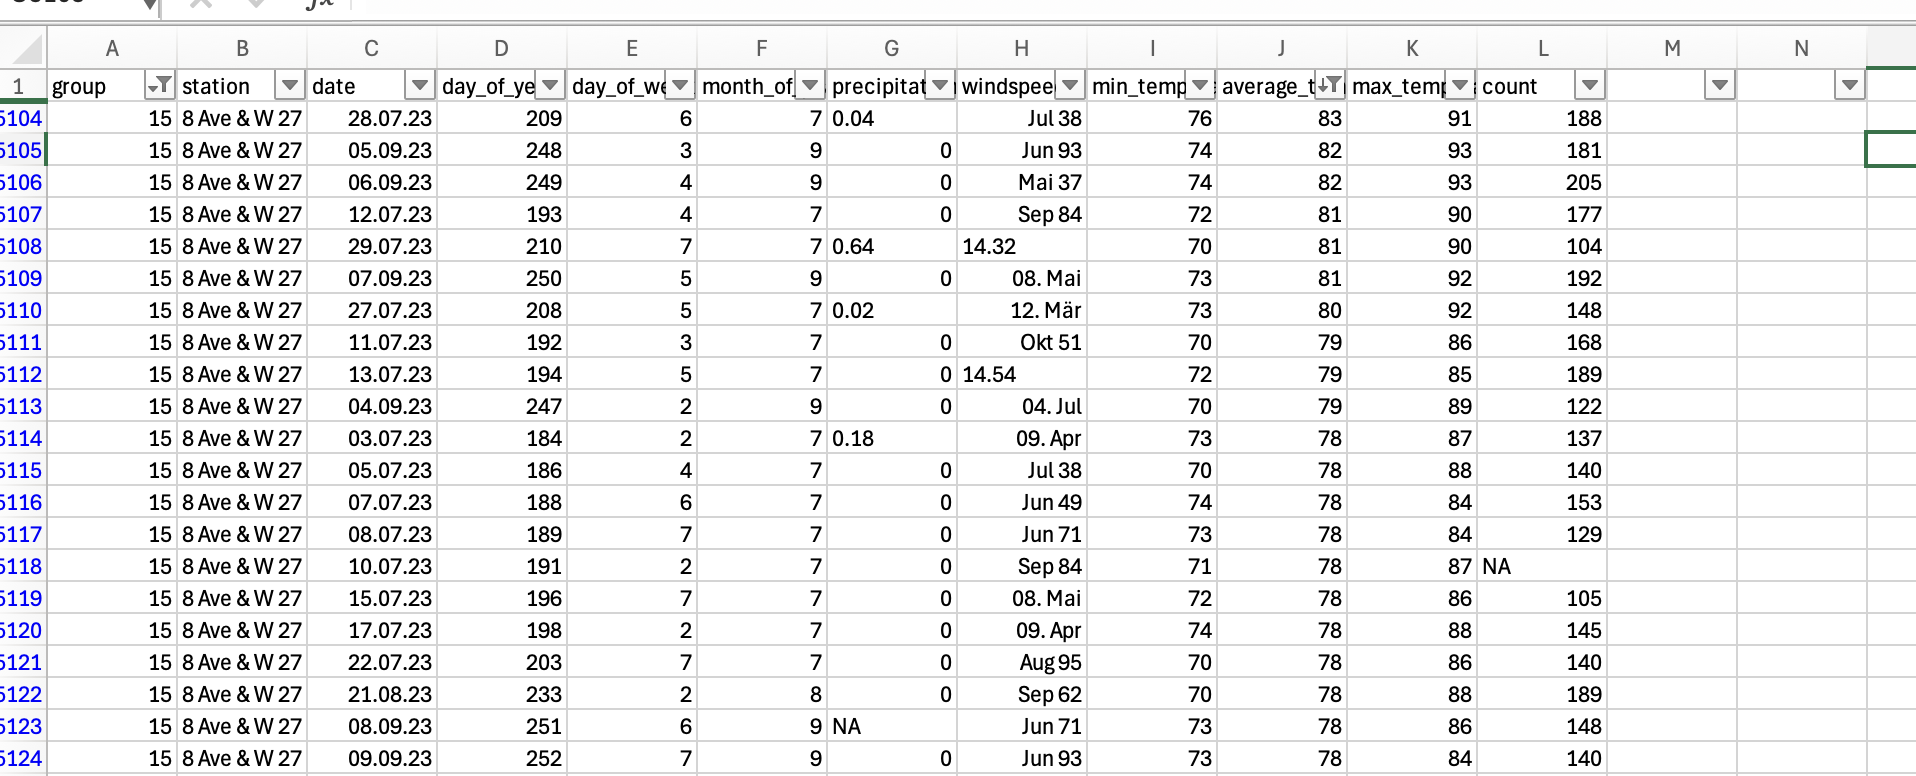
\includegraphics[width=1\linewidth]{Relevante Daten.png}
        \caption{Excel}
        \label{fig:Daten}
    \end{figure}
    
\item  Berechnen Sie für den Ihrer Gruppe zugeordneten Datenteil die höchste mittlere Temperatur. Die Angabe soll in Grad Celsius erfolgen. Beschreiben Sie, wie Sie vorgegangen sind und halten Sie auch das Berechnungsergebnis fest.

Die höchste mittlere Temperatur beträgt 83 Grad Fahrenheit, das sind ca. 28,333 Grad Celsius.
    
Mithilfe der Funktion: =MAX(J:J) oder =MAX(average\_temperature)
    
Excel ignoriert die NAs, ansonsten gibt es andere Möglichkeiten wie z.B. die Zeilen mit den NAs auszublenden und dann den Befehl $=MAX(J:J)$ einzugeben oder die Daten der Spalte zu sortieren (absteigend => oben dann der Wert 83). 

\end{enumerate}  
 \begin{figure} [h]
    \centering
    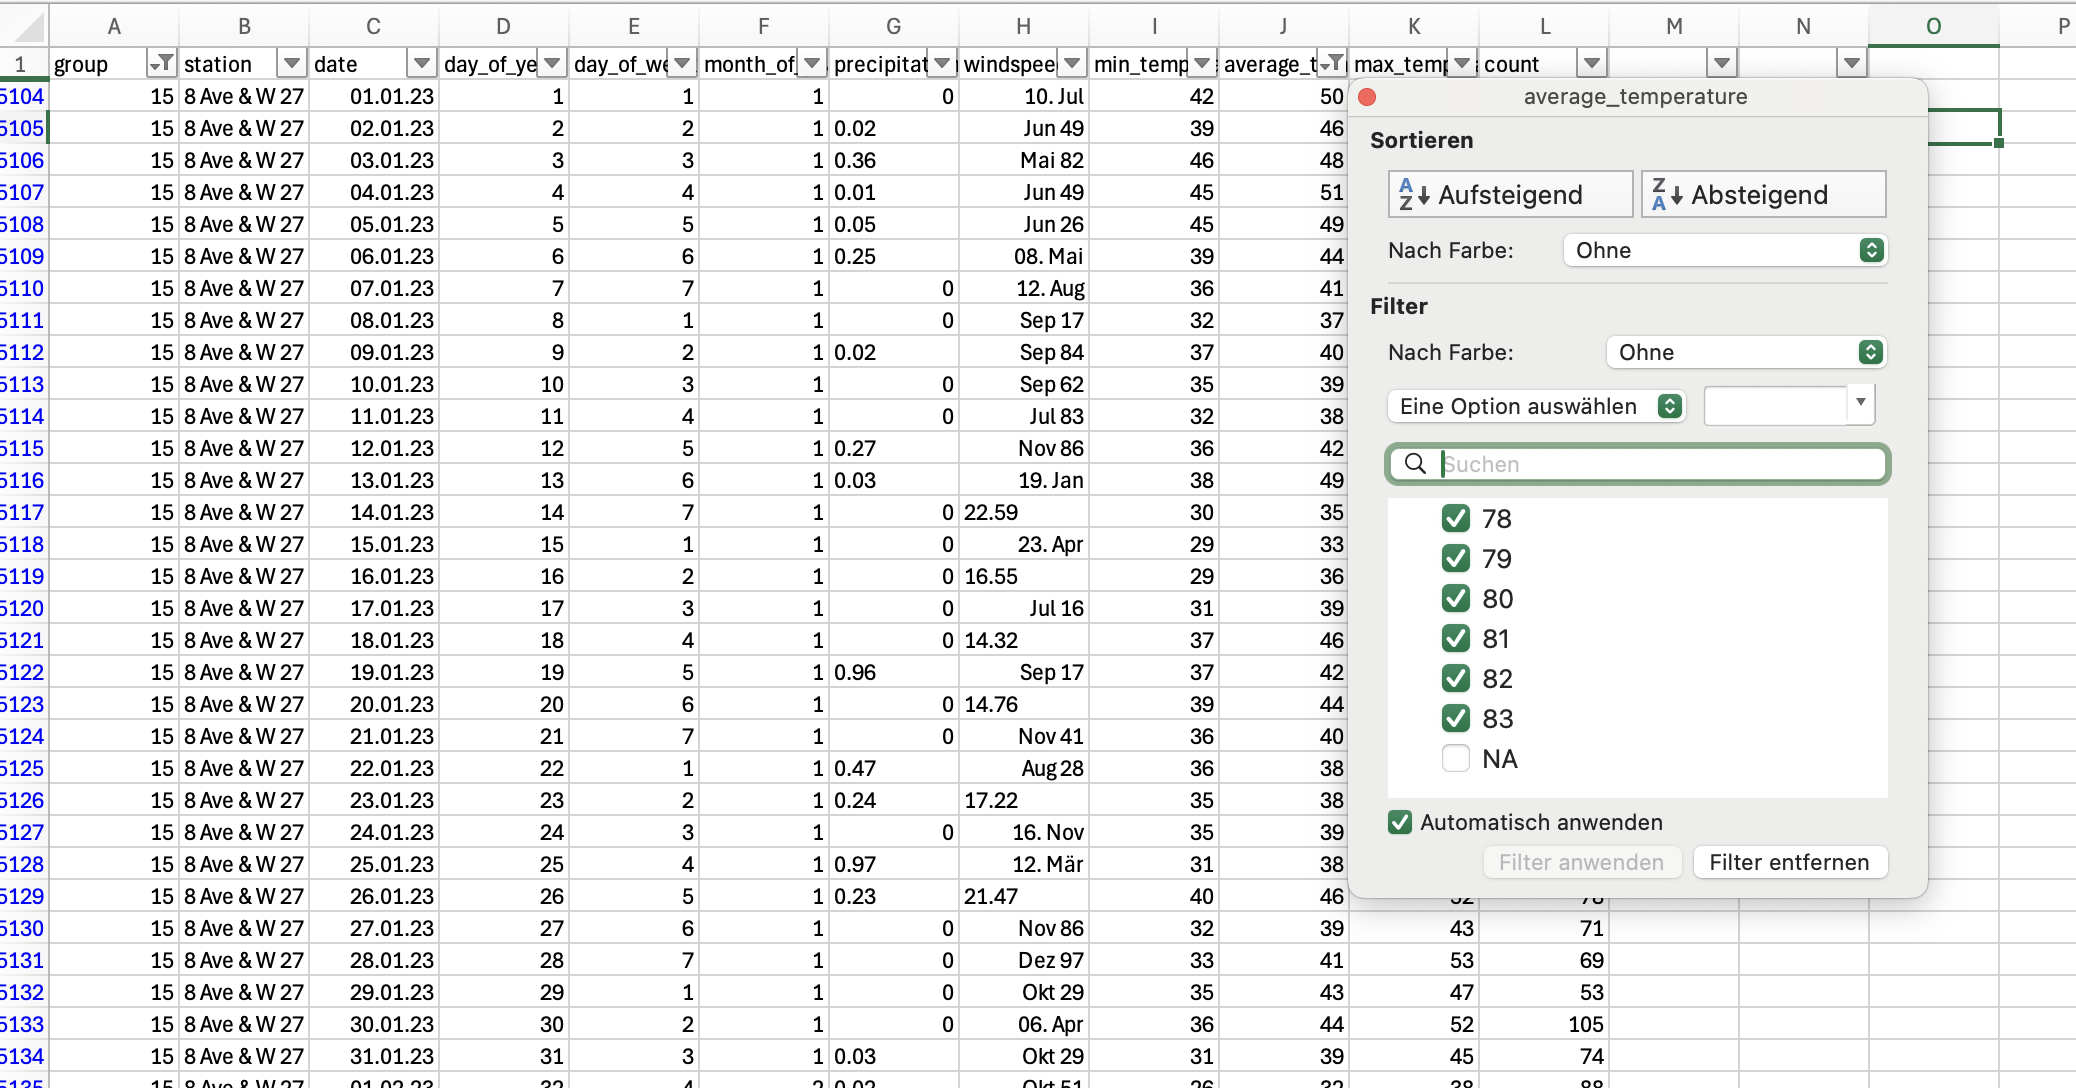
\includegraphics[width=0.6\linewidth]{Sort Filter.png}
    \caption{Sortieren und Filter}
    \label{fig:sort}
\end{figure}
\begin{figure} [h]
    \centering
    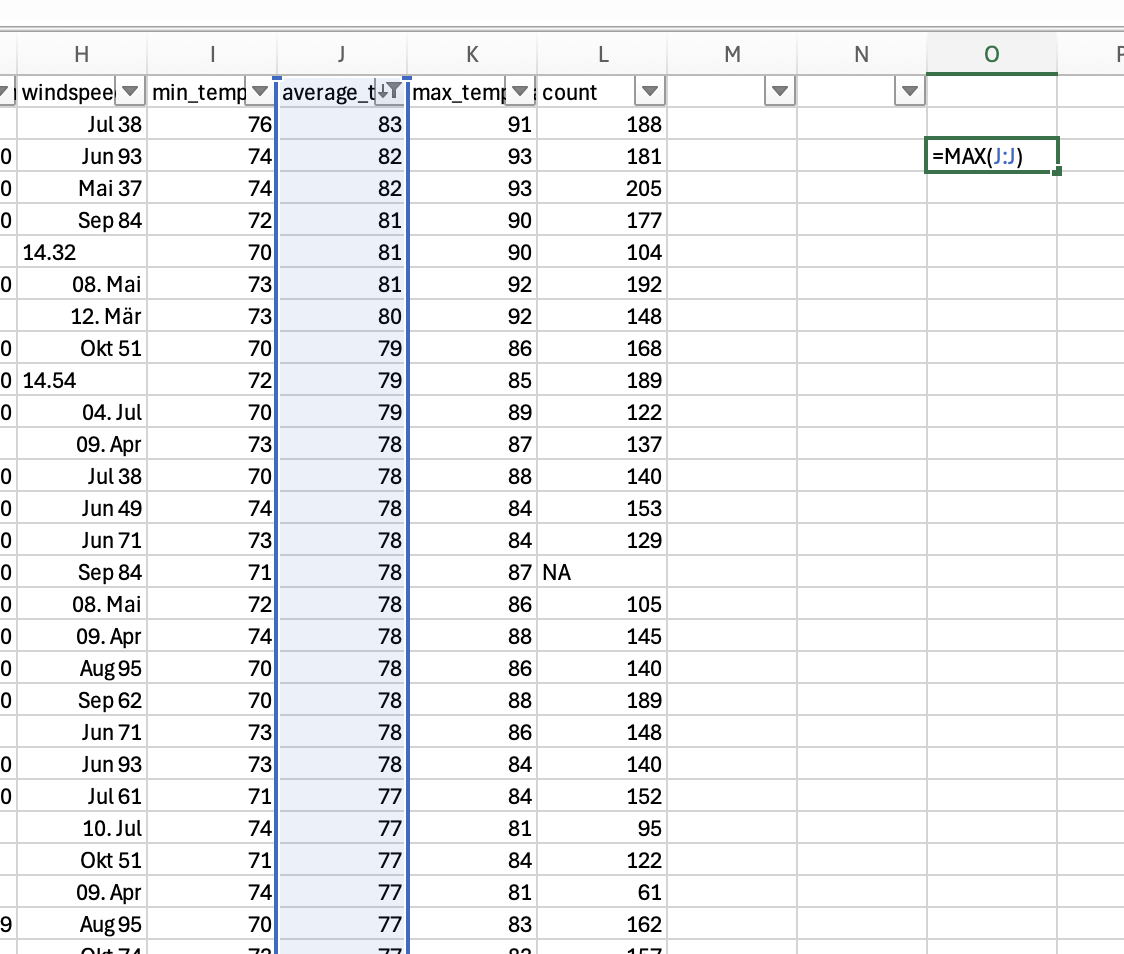
\includegraphics[width=0.8\linewidth]{Excel MAX.png}
    \caption{MAX-Befehl}
    \label{fig:Befehle}
\end{figure}


\subsection{Thema Datenhaltung}
\begin{enumerate}
\item Machen Sie sich dem in der Vorlesung vorgestellten DBMS SQLite (https://www.sqlite.org/) vertraut, auch im Hinblick auf mögliche Datentypen bei der Definition von Tabellen.

 SQL (Structured Query Language) ist eine standardisierte Programmiersprache, die verwendet wird, um Daten in relationalen Datenbanken zu verwalten und zu bearbeiten. Mit SQL können Daten erstellt, gelesen, aktualisiert und gelöscht werden.

 SQLite ist ein relationales Datenbankmanagementsystem (DBMS). Es wurde entwickelt, um Datenbanken effizient zu verwalten, ohne dass eine separate Serverinstallation oder -konfiguration erforderlich ist. 

 Unsere Gruppe hat für die folgenden Aufgaben mit Visual Studio Code (VSC) einem Code-Editor für viele Programmiersprachen gearbeitet.

\newpage
\item Entwerfen Sie im Abgabe-Dokument ein Datenbank-Schema im in der Vorlesung vorgestellten Format. Achten Sie dabei auf die 1. und 2. Normalform.

\underline{\textbf{Datenbank-Schema}}
\begin{figure}[h]
    \centering
    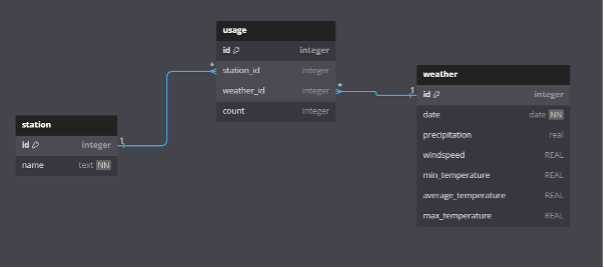
\includegraphics[width=0.7\linewidth]{Datenbank-Schema.png}
    \caption{Datenbank}
    \label{fig:Schema}
\end{figure}


Um die Daten logisch zu strukturieren und effizient zu speichern, wurde ein relationales Datenbankschema entworfen, das die Anforderungen der 1. Normalform (1NF) und 2. Normalform (2NF) erfüllt.

Zunächst wurde der gegebene Datensatz analysiert, um relevante Attribute und deren Abhängigkeiten zu identifizieren. Dabei wurde geprüft, welche Daten redundant gespeichert werden könnten und welche Attribute als Primärschlüssel oder Fremdschlüssel dienen können. Zusätzlich wurde darauf geachtet, dass die Attribute klar definiert und atomar sind, also jeweils nur einen Wert enthalten.
    
Das Schema besteht aus drei zentralen Tabellen: Station, Weather und Usage. Diese Tabellen repräsentieren die Hauptentitäten des Systems, nämlich Wetterstationen, Wetterdaten und die Nutzung von Stationen in Verbindung mit Wetterbedingungen.
    
\textit{\textbf{Tabelle: Station}}
    
Die Tabelle Station speichert Informationen zu den Wetterstationen, wie deren eindeutige Identifikationsnummer (id) und den Namen der Station (name). Sie ist unabhängig von den Wetterdaten, sodass Änderungen an der Stationsinformation keine Auswirkungen auf andere Tabellen haben. Durch die atomare Struktur dieser Tabelle erfüllt sie die Anforderungen der 1. Normalform, da jede Zelle nur einen einzelnen, unteilbaren Wert enthält. Redundanz wird vermieden, da jede Station nur einmal gespeichert wird und durch ihren Primärschlüssel (id) eindeutig referenziert werden kann.
\newpage    
\textit{\textbf{Tabelle: Weather}}
    
Die Tabelle Weather enthält detaillierte Wetterdaten, einschließlich des Datums (date), der Niederschlagsmenge (precipitation), der Windgeschwindigkeit (windspeed) sowie der minimalen, mittleren und maximalen Temperatur (min\_temperature, average\_temperature, max\_temperature). Jede Wetteraufzeichnung ist durch ihre eindeutige Identifikationsnummer (id) gekennzeichnet. Diese Tabelle erfüllt ebenfalls die 1. Normalform, da alle Attribute atomar sind und keine mehrwertigen oder zusammengesetzten Daten enthalten.
Die Wetterdaten sind von den Stationen entkoppelt, um sicherzustellen, dass Daten, die mehrfach verwendet werden könnten (z. B. Wetterbedingungen an einem bestimmten Tag für mehrere Stationen), nur einmal gespeichert werden. Dies vermeidet Redundanz und sorgt dafür, dass das Schema die 2. Normalform erfüllt: Alle Attribute in Weather hängen vollständig vom Primärschlüssel (id) ab.

\textit{\textbf{Tabelle: Usage}}
    
Die Tabelle Usage verbindet die Tabellen Station und Weather, indem sie die Nutzung von Stationen unter spezifischen Wetterbedingungen dokumentiert. Diese Tabelle enthält die Felder station\_id und weather\_id als Fremdschlüssel, die jeweils auf die Tabellen Station und Weather verweisen, sowie die Anzahl der Nutzungen (count).
Die Tabelle wurde so gestaltet, dass sie die Anforderungen der 2. Normalform erfüllt: Jedes Attribut hängt vollständig von ihrem Primärschlüssel (id) ab. Da station\_id und weather\_id Fremdschlüssel sind, wird sichergestellt, dass alle Informationen über Stationen und Wetterdaten aus den entsprechenden Tabellen stammen, wodurch Redundanz vermieden wird. So sind zum Beispiel die Wetterdaten für eine bestimmte Nutzung nicht mehrfach in der Tabelle Usagegespeichert, sondern werden über den Fremdschlüssel weather\_id referenziert. \\
    
      Station:
    \begin{itemize}
        \item id (Primärschlüssel) [int]
        \item name (Name der Statiion) [int]
    \end{itemize} 

    Weather:
    \begin{itemize}
        \item id (Primärschlüssel) [int]
        \item date (Datum des Wetters) [DATE]
        \item precipitation (Niederschlag) [REAL]
        \item windspeed (Windgeschwindigkeit) [REAL]
        \item min\_temperature (Minimale Temperatur) [REAL]
        \item average\_temperature(Mittlere Temperatur) [REAL]
        \item max\_temperature( Maximale Temperatur) [REAL]
    \end{itemize}
    
    Usage:
    \begin{itemize}
        \item id (Primärschlüssel) [int]
        \item station\_id (Fremdschlüssel auf Station) [int]
        \item weather\_id (Fremdschlüssel auf Weather) [int]
        \item count (Anzahl der Nutzungen) [int] \
        \end{itemize} 
        
\item Definieren Sie mit dem DDL-Teil von SQL die Tabellen. Halten Sie die SQL-Statements im Abgabe-Dokument fest.

 \begin{figure}[h]
     \centering
     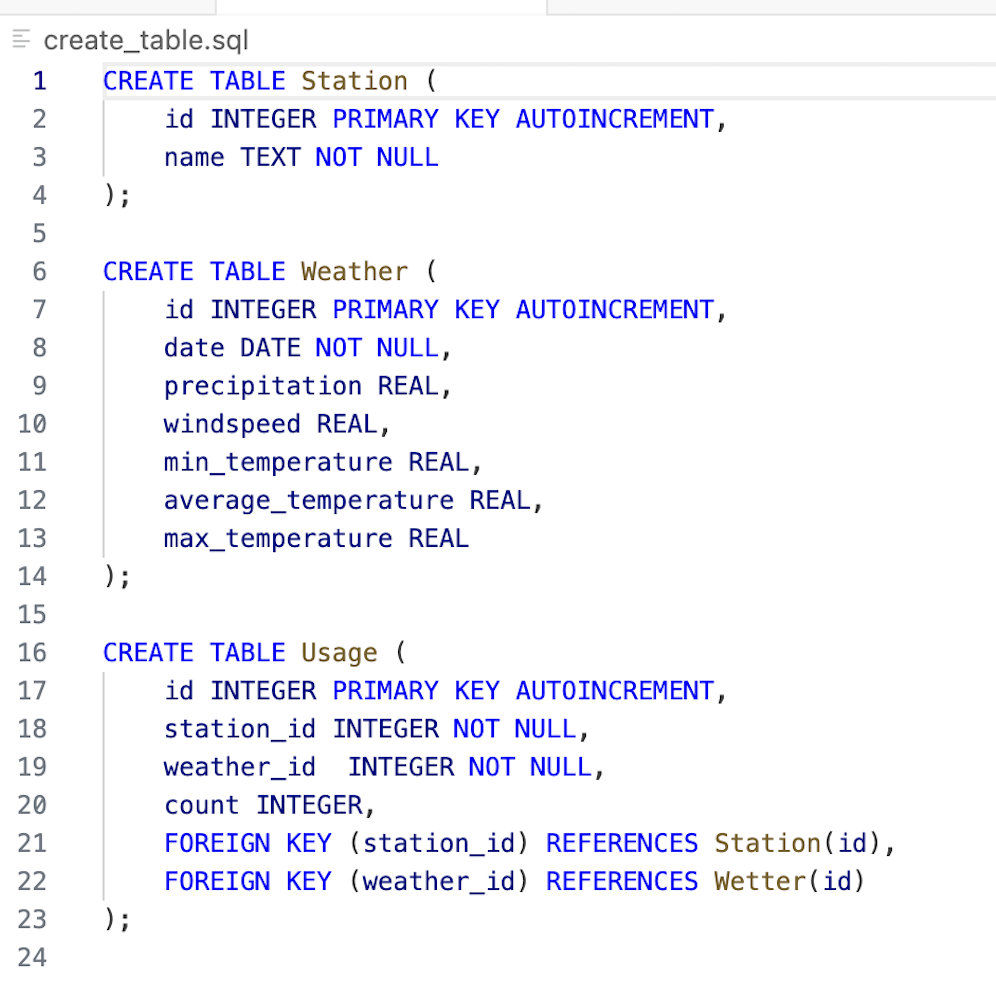
\includegraphics[width=0.6\linewidth]{Tabellen.png}
     \caption{Tabellen}
     \label{fig:SQL-Code}
 \end{figure}
   
\item Bereiten Sie den Datensatz so vor (per Programm oder Tabellenkalkulation), dass die Datensätze in die passenden Tabellen $importiert$ werden können. Beschreiben Sie Ihr Vorgehen.


\begin{figure}[h]
    \centering
    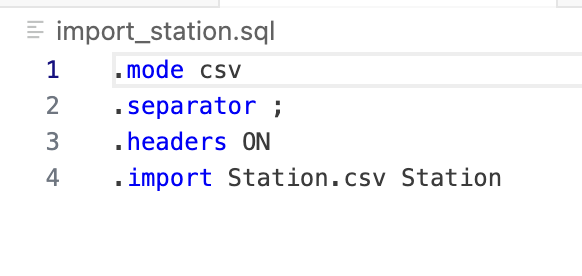
\includegraphics[width=0.5\linewidth]{import_station.png}
    \caption{Import der Daten der Station}
    \label{fig:SQL-Code2}
\end{figure}

\begin{figure}[h]
    \centering
    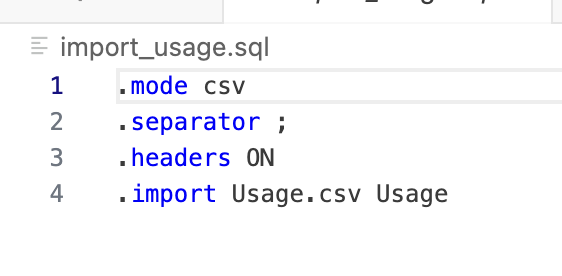
\includegraphics[width=0.5\linewidth]{import_usage.png}
    \caption{Import der Daten}
    \label{fig:SQL-Code3}
\end{figure}

\begin{figure}[h]
    \centering
    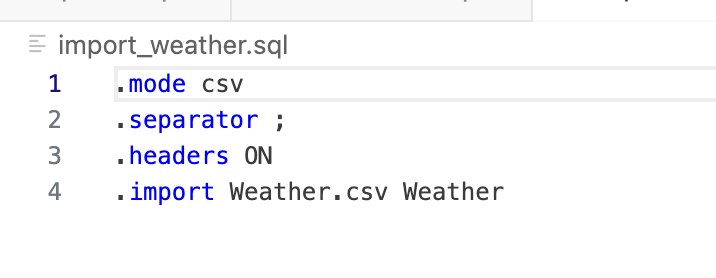
\includegraphics[width=0.6\linewidth]{import_weather1.png}
    \caption{Import der Wetterdaten}
    \label{fig:SQL-Code4}
\end{figure}

Wir haben die Daten in drei CSV-Dateien aufgeteilt: Station, Weather und Usage 

\item Formulieren Sie eine Abfrage, um aus den Ihrer Gruppe zugeordneten Daten die höchste mittlere Temperatur herauszufinden und halten Sie sowohl Abfrage als auch das Ergebnis (in Grad Celsius) fest. 

Datenbanken haben für Werte, die nicht existieren einen Begriff $NULL$. Wir dachten zuvor, dass wenn wir die leeren Zeilen in der CSV mit $NULL$ ersetzen, dass die Datenbank das richtig interpretiert. Leider wurde stattdessen NULL als Text gespeichert. Damit uns bei der Abfrage die höchste mittlere Temperatur nicht NULL angezeigt wird, mussten wir unsere importierte CSV-Datei erstmal updaten.
\end{enumerate}  

\begin{figure} [h]
    \centering
    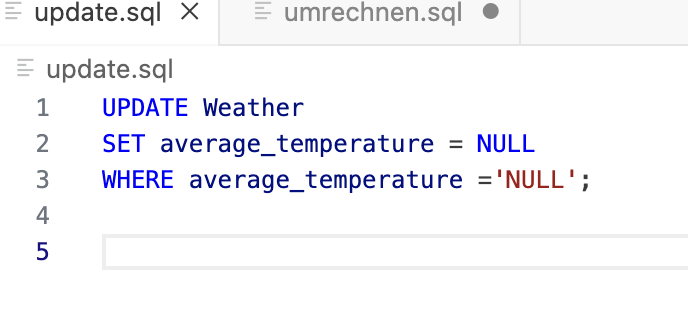
\includegraphics[width=0.6\linewidth]{update NAs.png}
    \caption{Update wegen NAs}
    \label{fig:SQL-Code4}
\end{figure}

\begin{figure}[h]
    \centering
    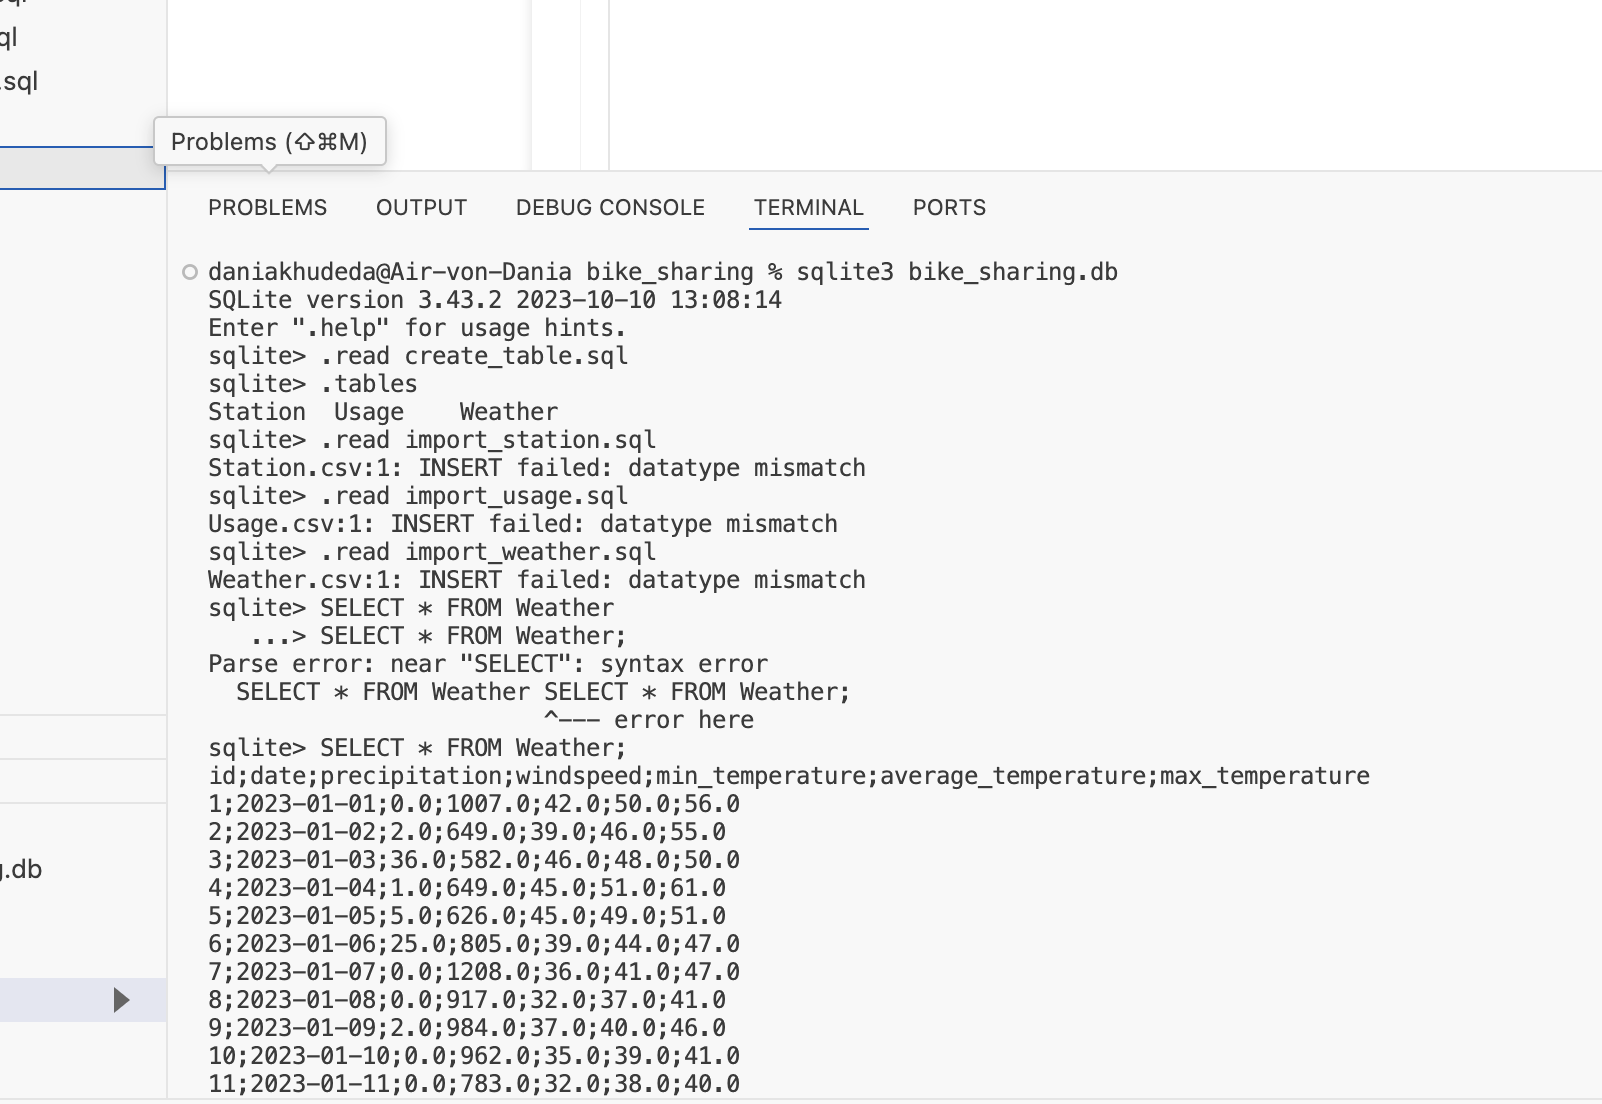
\includegraphics[width=0.7\linewidth]{Ausgeben.png}
    \caption{Ausgeben}
    \label{fig:Daten abrufen}
\end{figure}
\begin{figure} [h]
    \centering
    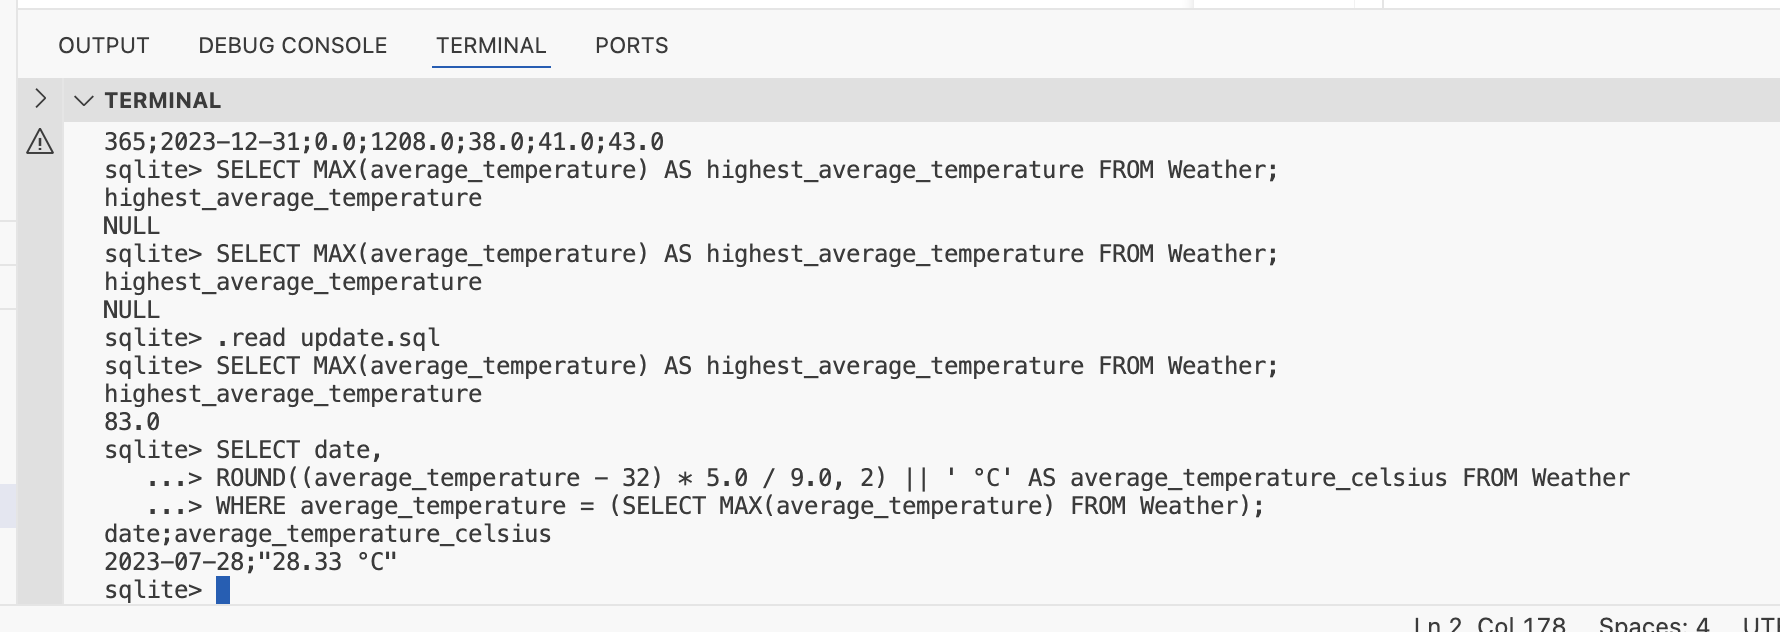
\includegraphics[width=1\linewidth]{Abfrage Temperatur.png}
    \caption{Höchste mittlere Temperatur in Grad Celsius}
    \label{fig:Abfrage}
\end{figure}
\begin{figure}
    \centering
    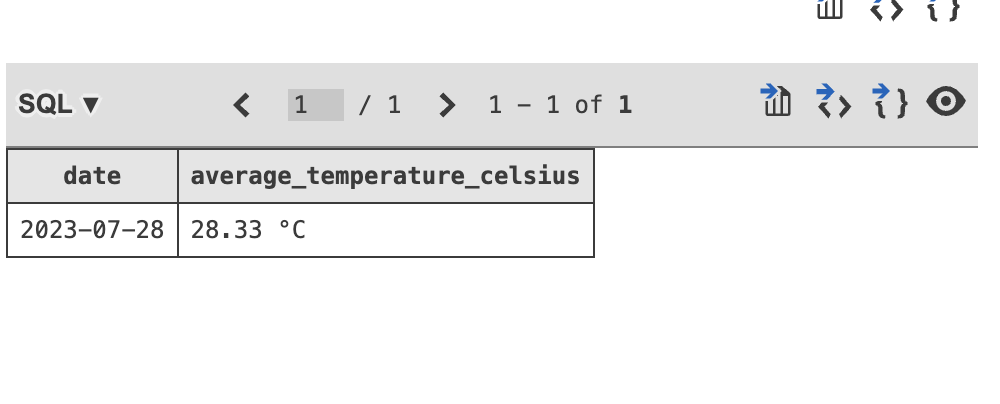
\includegraphics[width=0.5\linewidth]{Abfrage Bild.png}
    \caption{Temperatur}
    \label{fig:Temperatur}
\end{figure}
\begin{figure}[h]
    \centering
    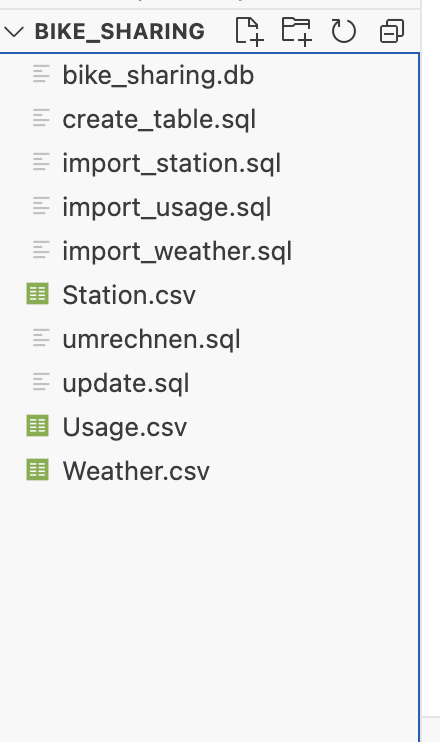
\includegraphics[width=0.35\linewidth]{Entwurf.png}
    \caption{Entwurf}
    \label{fig:Entwurf}
\end{figure}
\begin{figure}[b]
    \centering
    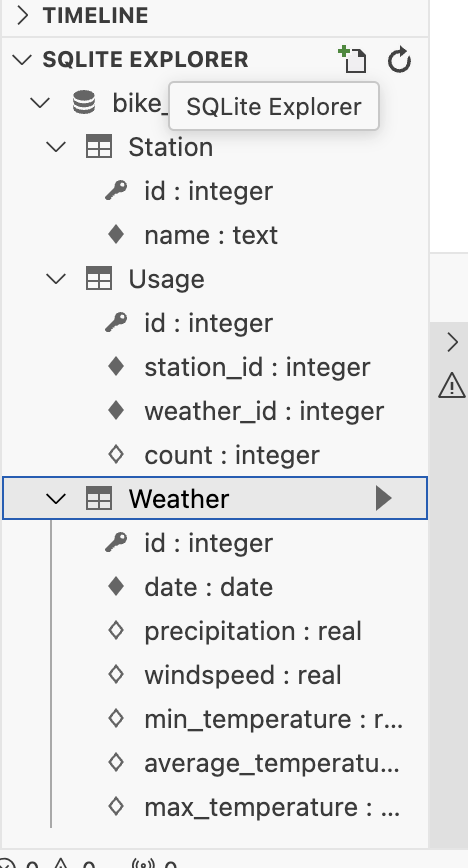
\includegraphics[width=0.35\linewidth]{Datenbank.png}
    \caption{Datenbank mit Tabellen}
    \label{fig:Datenbank}
\end{figure}
\clearpage
\subsection{GitHub}
Link für die Abgabe: https://github.com/Dania-Khudeda/Abgabe-1.git

\clearpage
\bibliographystyle{plain}
\bibliography{references}
\end{document}
